% WORKING OFF-LINE : if you are interested to install "latex packages" and an off-line editor, please refer to:

% DISTRUBUTIONS
% https://www.latex-project.org/get/#tex-distributions
% ....

% EDITORS (search on google)
% TexStudio
% TexWorks
% TexShop
% ...


% Keep in mind that the entry order of packages might be relevant. 
% packages documentation on https://ctan.org
% miscellaneous https://en.wikibooks.org/wiki/LaTeX
\documentclass[11pt,a4paper,oneside]{article}
\usepackage[T1]{fontenc} 
\usepackage[utf8]{inputenc}
\usepackage[main=english]{babel}
\usepackage{graphicx} % 1pt = 0.035146cm
\graphicspath{{Figures/}}
\usepackage[justification=default]{subfig} %Manage sub-figures 
\usepackage[update]{epstopdf}
\usepackage[labelfont=bf]{caption}
\usepackage{titlesec} % Allows customization of titles
\usepackage{booktabs}
\usepackage[textwidth = 450pt,top = 80pt, bottom = 60pt]{geometry}
\usepackage{xcolor}
\usepackage{threeparttable}
\usepackage{soul}
\newcommand{\hlc}[2][yellow]{{\sethlcolor{#1}\hl{#2}}}
%--------------------------------------------------------------------------------
%       MATH PACKAGES
%--------------------------------------------------------------------------------
\usepackage{amsmath}
%\usepackage{mathtools}
\usepackage[leqno,fleqn,intlimits]{empheq}
\usepackage{bm}
%\usepackage{amssymb}
\renewcommand{\vec}[1]{\mathbf{#1}} % \mathbf merge roman and bold
\newcommand{\mathbi}[1]{\bm{\textbf{\em #1}}}
\usepackage{empheq}
\newcommand{\di}[2]{\frac{\mathrm{d} #1}{\mathrm{d} #2}}
\DeclareMathOperator{\vect}{vec}
%--------------------------------------------------------------------------------
%       BIBLIOGRAPHY PACKAGES
%--------------------------------------------------------------------------------
\usepackage{csquotes}
\usepackage[sorting=nyt,%
sortcites=true,%
bibencoding=ascii,%
autopunct=true,%
hyperref=true,%
language=auto,%
%backref=true,%
url=false,%
%maxcitenames=10,%
%minbibnames = 20,%
maxbibnames = 2,%
giveninits, 
natbib = false,
isbn=false,%
backend=biber]{biblatex}
\addbibresource{bibliograhy_assignment.tex}
%--------------------------------------------------------------------------------
%       MISCELLANEA
%--------------------------------------------------------------------------------
\usepackage[]{hyperref}
\usepackage{cleveref}
%%% CREF setup
\crefname{equation}{Eq.}{Eqs.}
\crefname{table}{Table}{Tables}
\crefname{figure}{Figure}{Figures}
\crefname{section}{Section}{Sections}

%--------------------------------------------------------------------------------
%       TITLE SECTION
%--------------------------------------------------------------------------------
\title{Guidelines for MSAS reports in \LaTeX} % Article title
\author{\large C.\ Giordano, V.\ Franzese}
\date{}

%--------------------------------------------------------------------------------
% HEADING packages
\usepackage{fancyhdr} % Headers and footers control
\setlength{\headheight}{30.62pt}
\pagestyle{fancyplain} % Defines a new header for all pages (absolutely all pages, use fancy to exclude title-page and chapters, if book class is used) 
\fancyhf{} % clears the header and footer, otherwise the elements of the default "plain" page style will appear
%
\lhead{Guidelines for MSAS reports in \LaTeX}
\rhead{\vspace{-0.5cm}
\includegraphics[width=0.3\textwidth]{newlogo.eps}}
\lfoot{TA: C.\ Balossi, S.\ Borgia}
\rfoot{\thepage}

%--------------------------------------------------------------------------------
%       BEGIN DOCUMENT
%--------------------------------------------------------------------------------
\begin{document}
\maketitle
\thispagestyle{fancy}
\section{Guidelines}%\label{sec:introduction}
This document gives some advices in order to write the MSAS reports in \LaTeX, e.g., packages, commands, and  stylistic guidelines. The reader is referred to the \emph{source code} in \verb|main.tex|. 

The topics described are:
%
\begin{itemize}
    \item Tables (\cref{subsec:tables});
    \item Figures and file formats (\cref{subsec:figures});
    \item Equations (\cref{subsec:equations});
    \item Bibliography (\cref{subsec:biblio}).
\end{itemize}

Part of the material that follows is re-worked starting from guidelines produced by the American Institute of Aeronautics and Astronautics (AIAA) for journal authors (website: \url{https://www.aiaa.org/journal-authors/#Prepare}).

There are a multitude of user's guides for document writing in \LaTeX, so feel free to use one of these; good examples \url{https://www.latex-project.org}, \url{https://tex.stackexchange.com}, and \url{http://www.lorenzopantieri.net/LaTeX_files/ArteLaTeX.pdf} (in Italian).


%------------------------------------------------------------------------
%------------------------------------------------------------------------
\subsection{Tables}\label{subsec:tables}
Referring to a table should happen before placement of the table itself.
All tables are numbered and include a caption (definitive title) at the top. Each table must be cited in the text in numerical order and \emph{before} the table is placed in the text; table footnotes may be used to define acronyms or other terminology within the table (advice: use \emph{threeparttable} package). Do not use border lines or vertical rules between columns, but do use a double rule above and below the body of each table and a single rule under the column headings.

\medskip %optional
\noindent \textcolor{blue}{YES! Cite before the table: \cref{tab:exampleoftable} outlines the recommended style for editing table.}
%
\begin{table}[htb]
    \centering
    \begin{threeparttable}
        \caption{\label{tab:exampleoftable}Example of table.}
        \begin{tabular}{lcr}
            \toprule
            \toprule
            T$_{max}$, N&  v, m/s$^2$& x, m\\ 
            \midrule
            3\tnote{$\dagger$}&13.57 $\times 10^{2}$& 1.333$\times 10^{-3}$\\
            2&34.78E+03& 0.666E-04\tnote{$\star$}\\
            \bottomrule
            \bottomrule
        \end{tabular}
        \begin{tablenotes}
            \footnotesize
            \item[$\dagger$] example of footnote
            \item[$\star$] example, retrieved from \cite{zhang2015low}.
        \end{tablenotes}
    \end{threeparttable}
\end{table}
%
\\
\noindent \textcolor{red}{NO! Cite after the table: \cref{tab:exampleoftable} outlines the recommended style for editing table.}

%
%------------------------------------------------------------------------
%------------------------------------------------------------------------
\subsection{Figures}\label{subsec:figures}
All figures are numbered and include a caption (definitive title) at the bottom. Each figure must be cited in the text in numerical order and \emph{before} it is represented.
You may position them within the text of your article close to where they are cited. 

\medskip
\noindent \textcolor{blue}{YES! Reference before the figure: \cref{fig:exampleoffigure} shows the overleaf symbol.}
\\
\begin{figure}[htb]
    \centering
    
\includegraphics[width=0.3\textwidth]{overleaf_logo.png}
    \caption[]{\label{fig:exampleoffigure} Example of figure.}
\end{figure}
\\
\noindent \textcolor{red}{NO! Reference after the figure: \cref{fig:exampleoffigure} shows the overleaf symbol.}
%------------------------------------------------------------------------
\subsubsection{Image file formats}\label{subsubsec:imagefileformats}
Note the difference among different image file formats in \cref{fig:possibleimagefileformats} (zoom-in the complied figures in main.pdf). If possible, use the \verb|.eps| format. For example, in MATLAB, use the ``export setup'' MATLAB command when you save an image. 

\noindent Note also the different line style of the legend: you should produce a legend that is color agnostic, i.e., legend adapted for black and white papers or color blind readers. When figures are retrieved from the literature, cite the source (see \cref{fig:EPSimage}).
\begin{figure}[htp]
    \centering
    \subfloat[][JPG image\label{fig:jpegimage}]
    {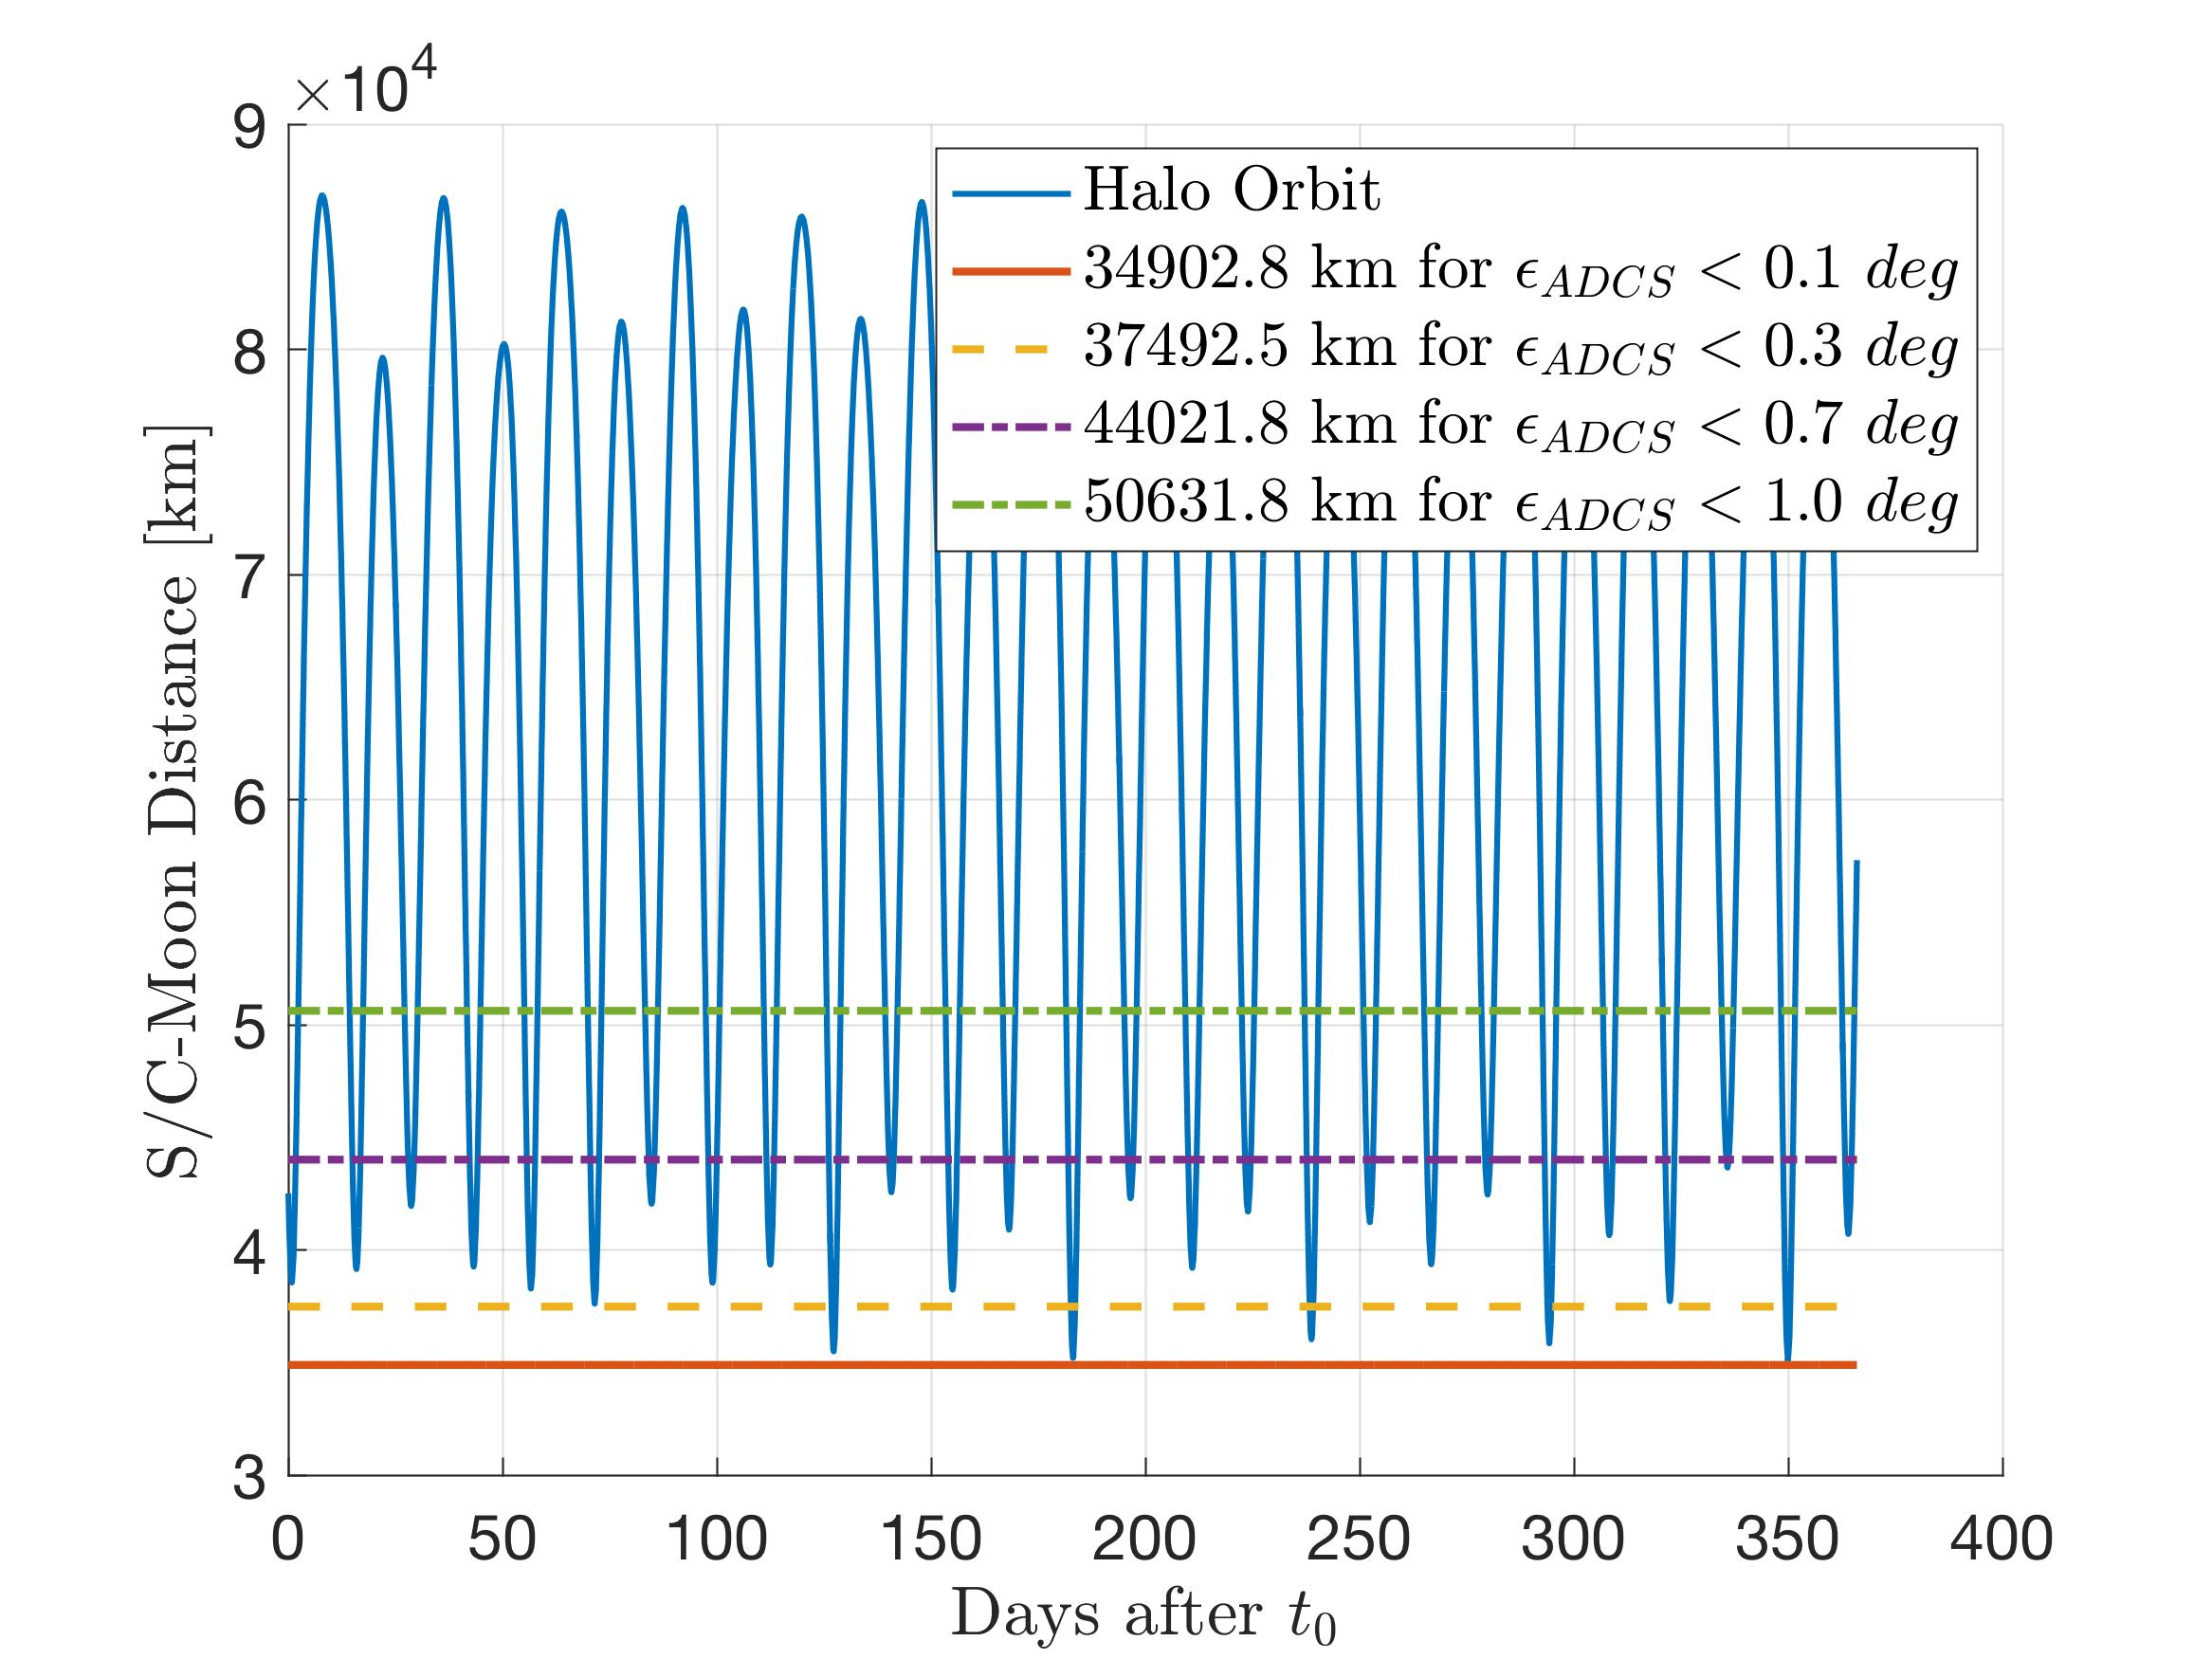
\includegraphics[width=0.4\textwidth]{jpgfigure.jpg}}\quad
    \subfloat[][PNG image\label{fig:ongimage}]
    {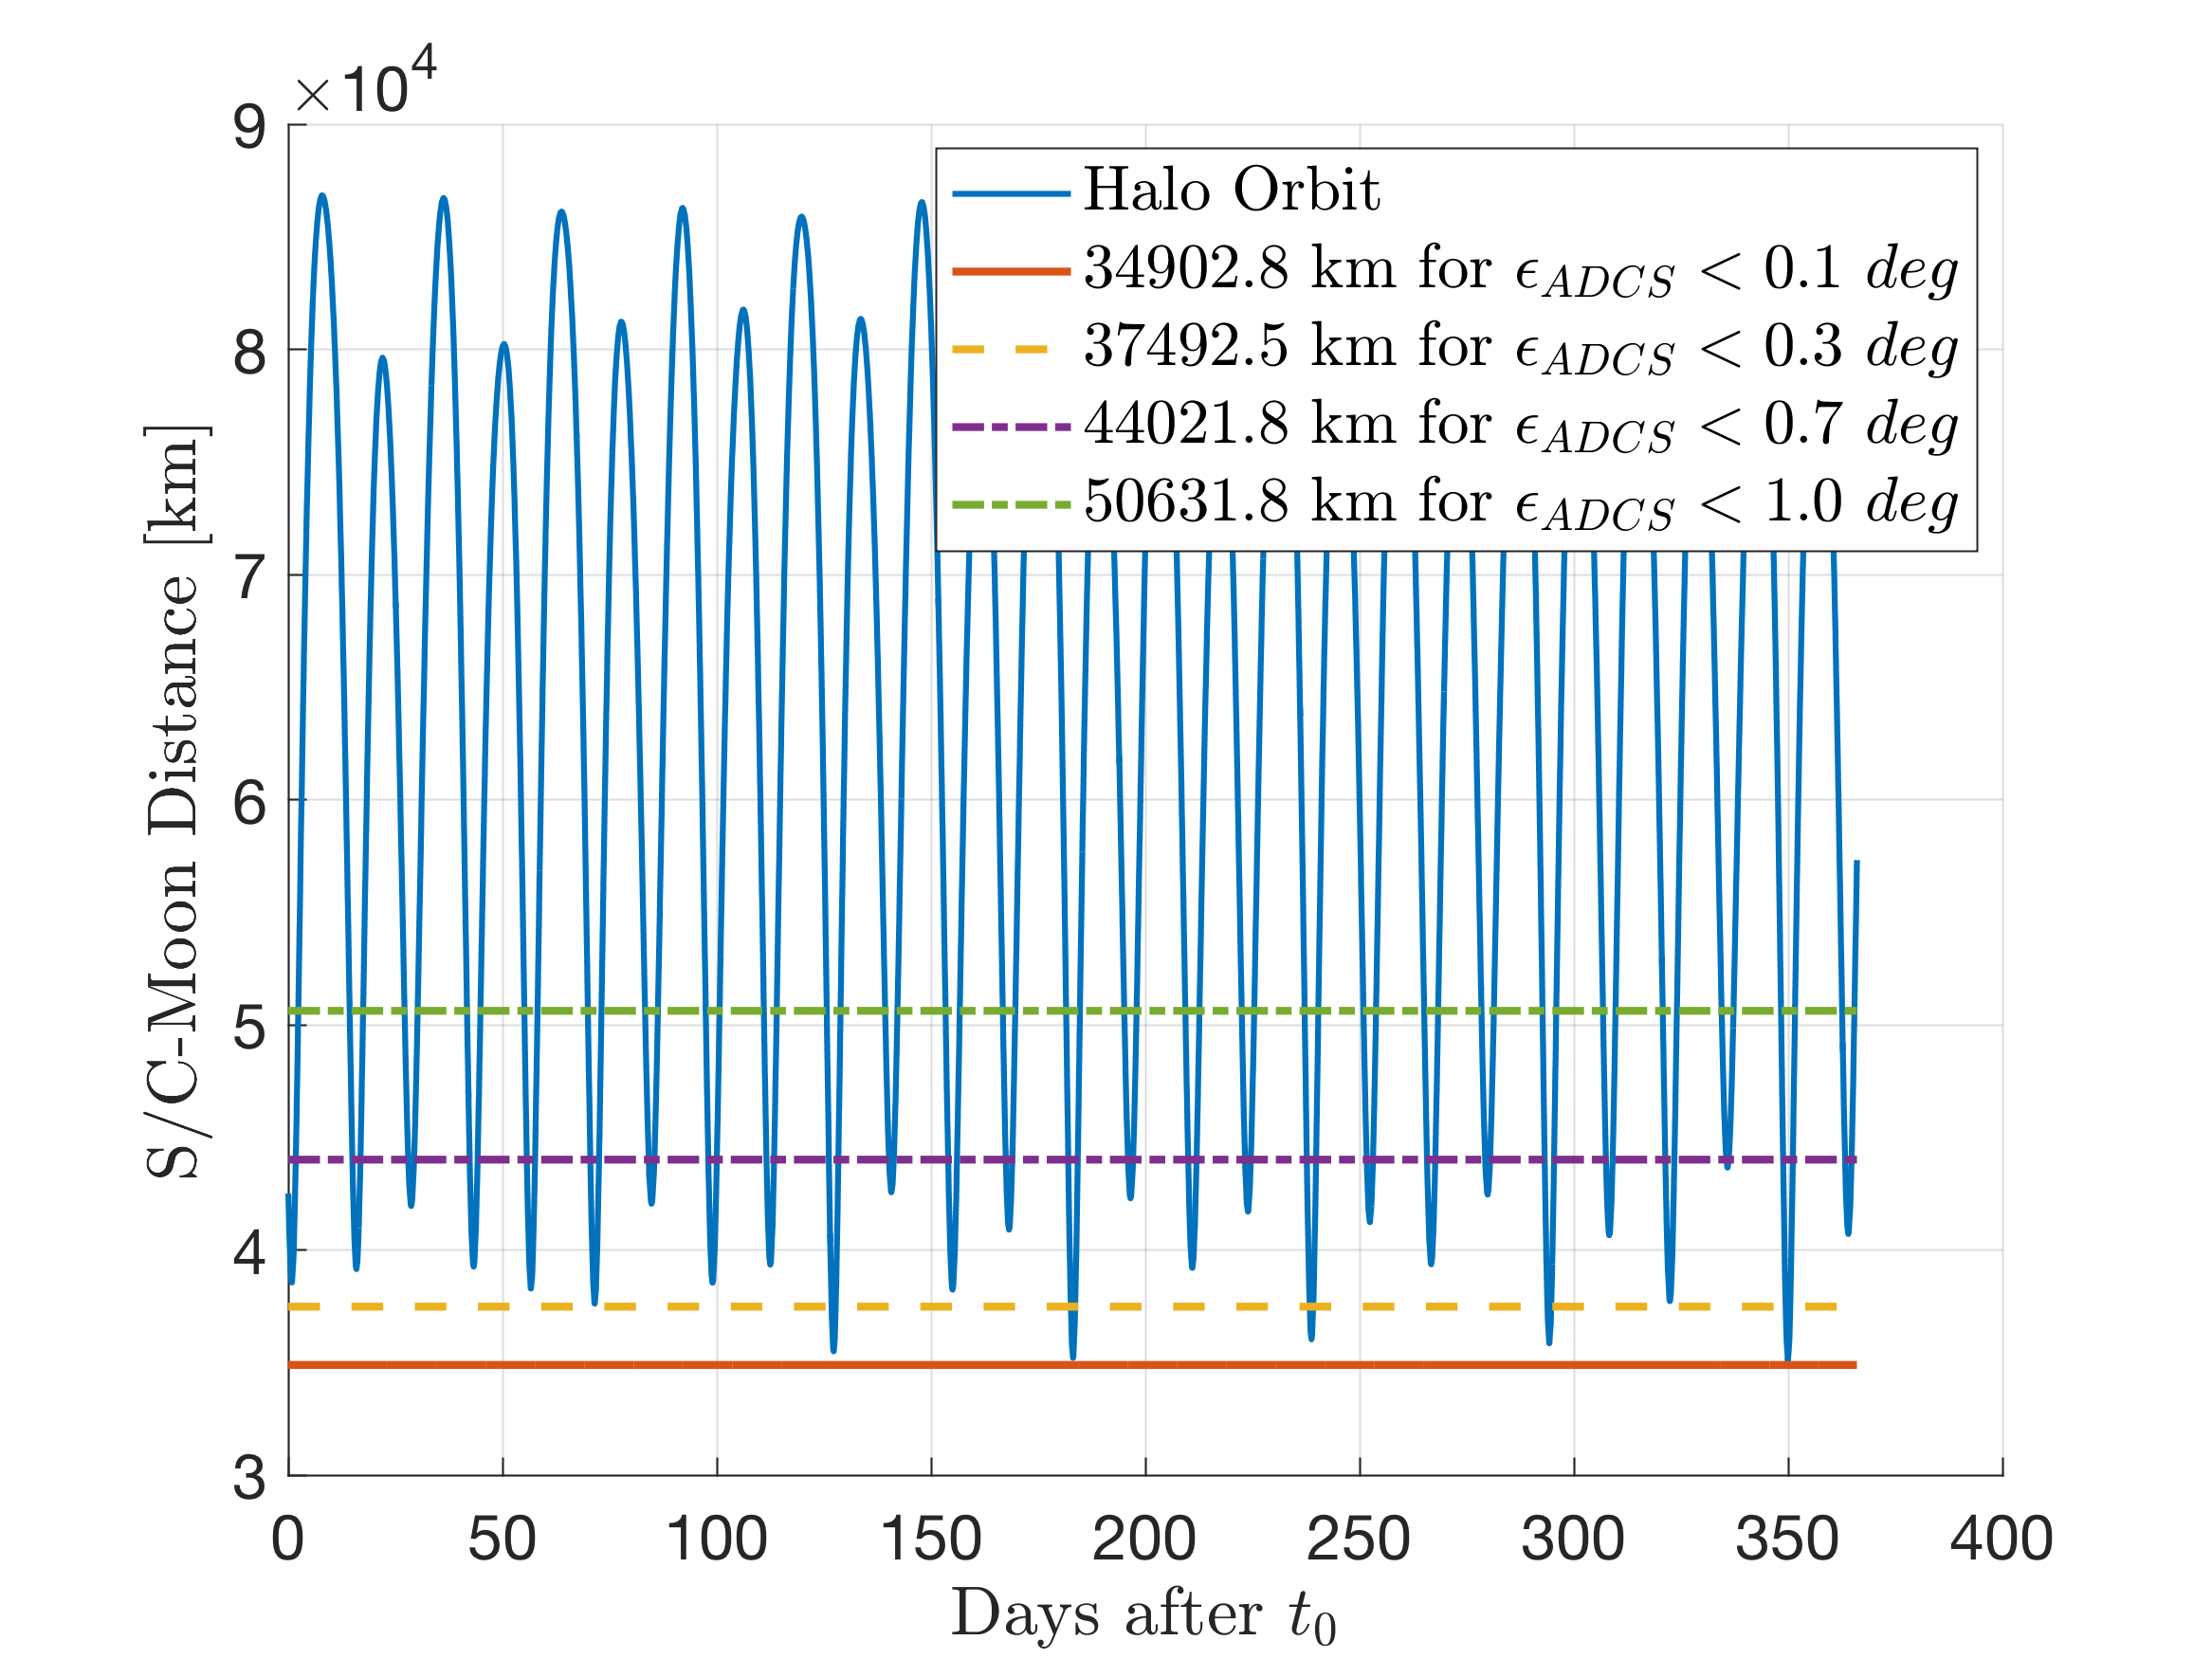
\includegraphics[width=0.4\textwidth]{pngfigure.png}}\\
    \subfloat[][EPS image, retrieved from \cite{lumiosysnova}.\label{fig:EPSimage}]
    {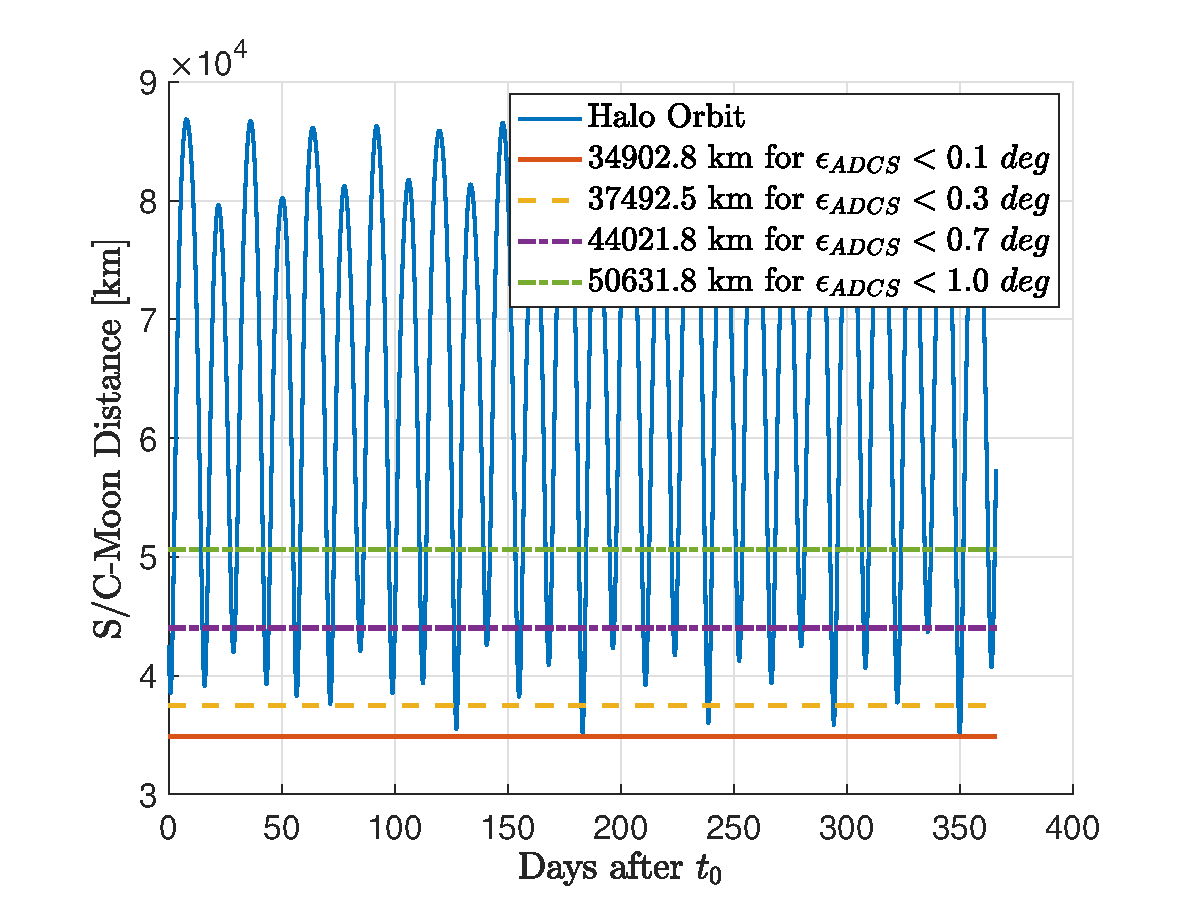
\includegraphics[width=0.4\textwidth]{epsfigure.eps}}
    \caption{Possible image file formats.\label{fig:possibleimagefileformats}}
\end{figure}

%------------------------------------------------------------------------
%------------------------------------------------------------------------
\subsection{Equations}\label{subsec:equations}
Keep equations simple, and avoid unusual characters or symbols. Tips: 1) avoid using under-barred symbols, 2) Avoid using multiple dot accents (in excess of two). Use boldface symbol for vector quantities and capital letter for matrices. 
Contrary to what stated for figures and tables in the previous Sections, equations can be referred to also \emph{after} they are presented.
\noindent A list of equations with various layout is represented hereinafter: try to adapt the style to what you are writing about. For example, if the canonical state space representation is needed for a system of equations, a good idea is to align the right-hand side of each variable.

\begin{equation}
    \mathbi{M}~\ddot{\vec{x}}+\mathbi{C}~\dot{\vec{x}}+\mathbi{K}\,\vec{x} = \mathbi{F}
    \label{eq:massspringdamper}
\end{equation}
%
\begin{align}
    &3\vec{x}+4\vec{y} = \vec{c}\label{eq:alignone}\\
    &\vec{z} = \vec{f}\left(\vec{x},\,\vec{y}\right)\label{eq:aligntwo}
\end{align}
%
\begin{empheq}[left=\empheqlbrace]{align}
  2x+y    =  1 \label{eq:bracealignone}\\
  8x\,y    = 12 \label{eq:bracealigntwo}\\
  12 x/c = 10 \label{eq:bracealigthree}
\end{empheq}
%
\begin{subequations}
    \begin{align}
        \vec{\dot{x}} &= \vec{f}\left(\vec{x},\vec{y}\right) \label{eq:subalignone}\\
        \vec{\dot{y}} &= \vec{g}\left(\vec{x},\vec{y}\right)\mathbf{x} \label{eq:subaligntwo}
    \end{align}
\end{subequations}

In some limited cases (e.g. intermediate steps of a demonstration), equations can be also unreferenced:

\begin{equation*}
    f(x)=f(x_0)+\frac{f'(x_0)}{1!}(x-x_0)+\frac{f''(x_0)}{2!}(x-x_0)^2+o\left((x-x_0)^2\right)
\end{equation*}

$$\vect\left(\di{\sqrt{\mathbi{A}}}{x}\right)=\left(\sqrt{\mathbi{A}}~^T\oplus\sqrt{\mathbi{A}}\right)^{-1}\vect\left(\di{\mathbi{A}}{x}\right)$$

\subsection{Bibliography}\label{subsec:biblio}
All references must be numbered and cited in numerical order in the text. The original source of a work mist be cited, not a secondary source. The Digital Object Identifier should be incorporated into every reference whenever possible.

\printbibliography

\end{document}
%--------------------------------------------------------------------------------
%       END DOCUMENT
%--------------------------------------------------------------------------------